In this chapter we'll describe the results we obtained by applying the \textbf{SI}, \textbf{SIS}, \textbf{SIR},
and \textbf{Threshold} diffusion models both on the crawled data and on the synthetic graphs (Erdős–Rényi and
Barabási–Albert) generated from the original one. In each section, a comparison between the three networks will be
provided both for the trend and for the prevalence of every model.

\section{SI model} % (fold)
\label{sec:si_model}
    \begin{figure}[H]
        \centering
        \begin{subfigure}{0.45\textwidth}
            \resizebox{\textwidth}{!}{
                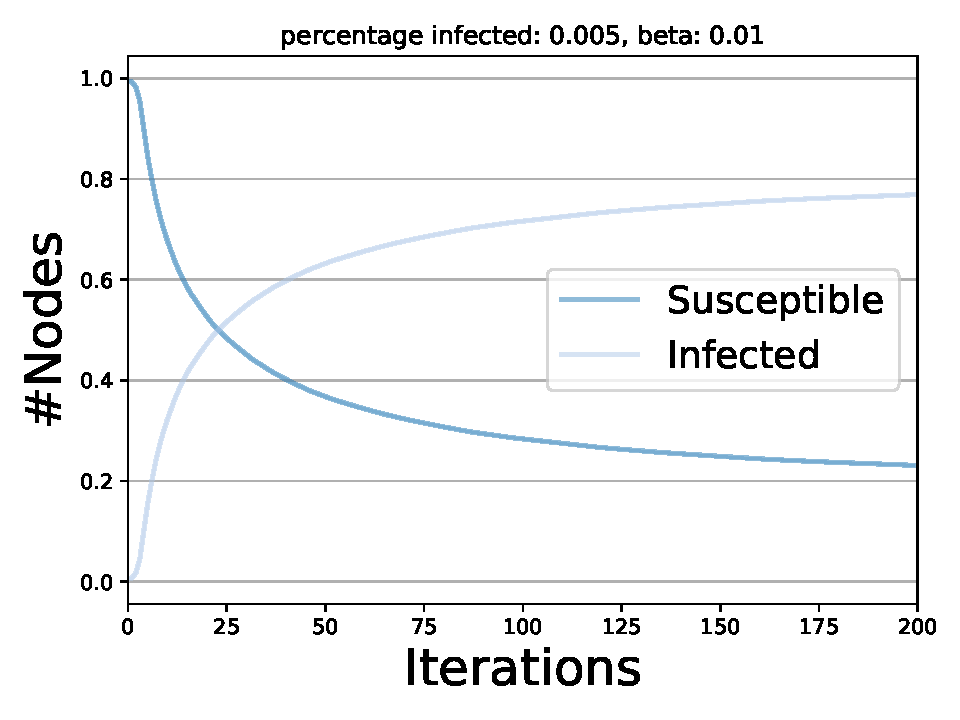
\includegraphics{images/spreading/si/diffusion.pdf}

            }
            \caption{}
            \label{diff_si}
        \end{subfigure}
        \begin{subfigure}{0.45\textwidth}
            \resizebox{\textwidth}{!}{
                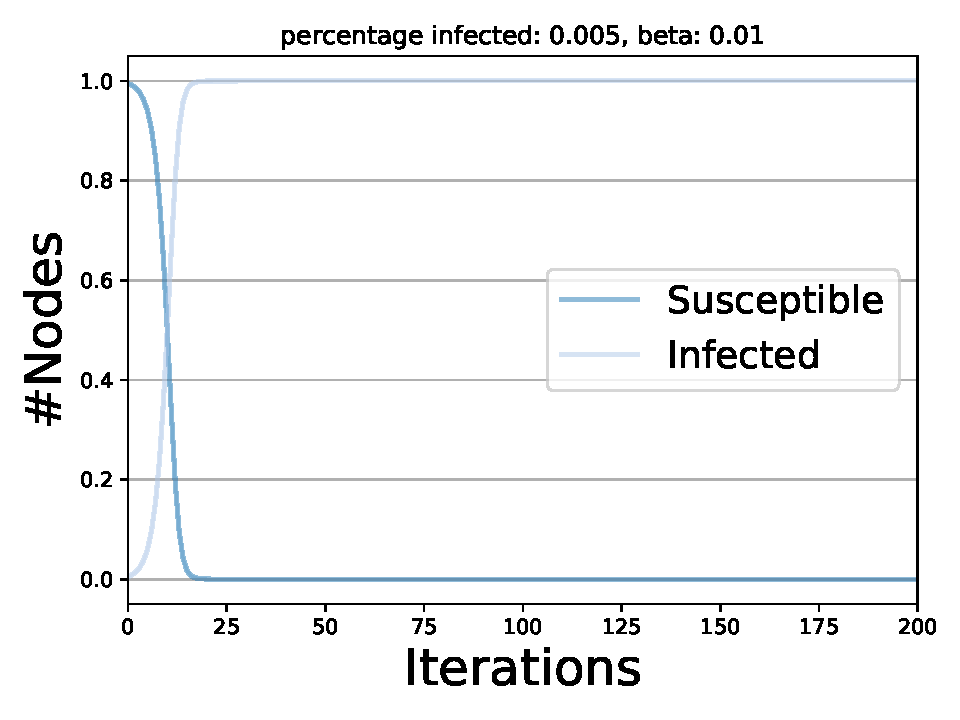
\includegraphics{images/spreading/si/diffusion_er.pdf}
            }
            \caption{}
            \label{diff_si_er}
        \end{subfigure}
        \begin{subfigure}{0.45\textwidth}
            \resizebox{\textwidth}{!}{
                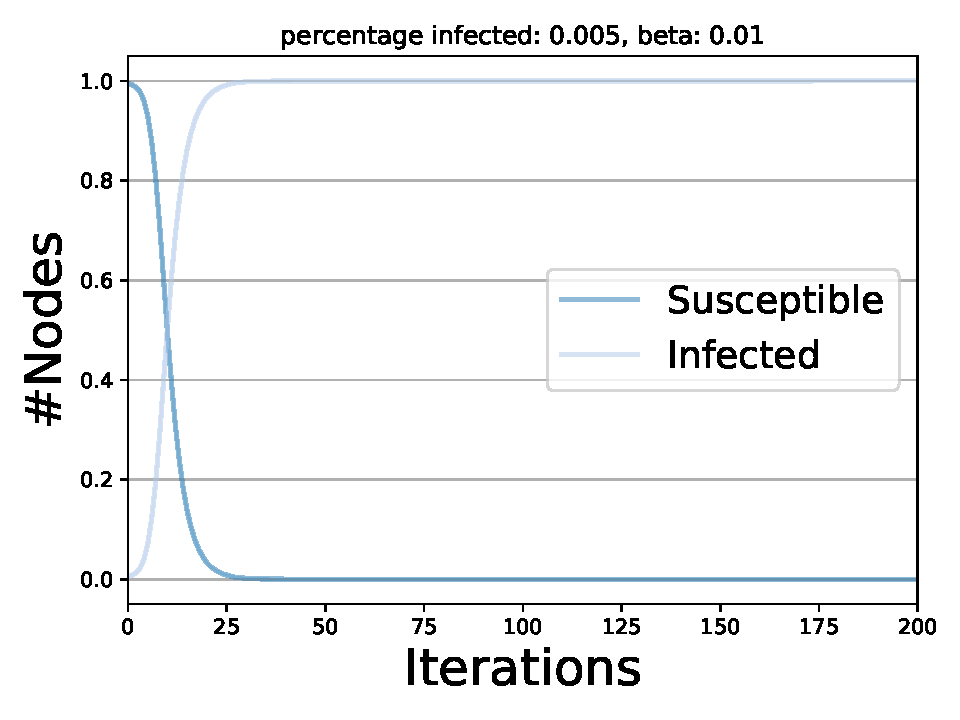
\includegraphics{images/spreading/si/diffusion_ba.pdf}
            }
            \caption{}
            \label{diff_si_ba}
        \end{subfigure}
        \begin{subfigure}{0.45\textwidth}
            \resizebox{\textwidth}{!}{
                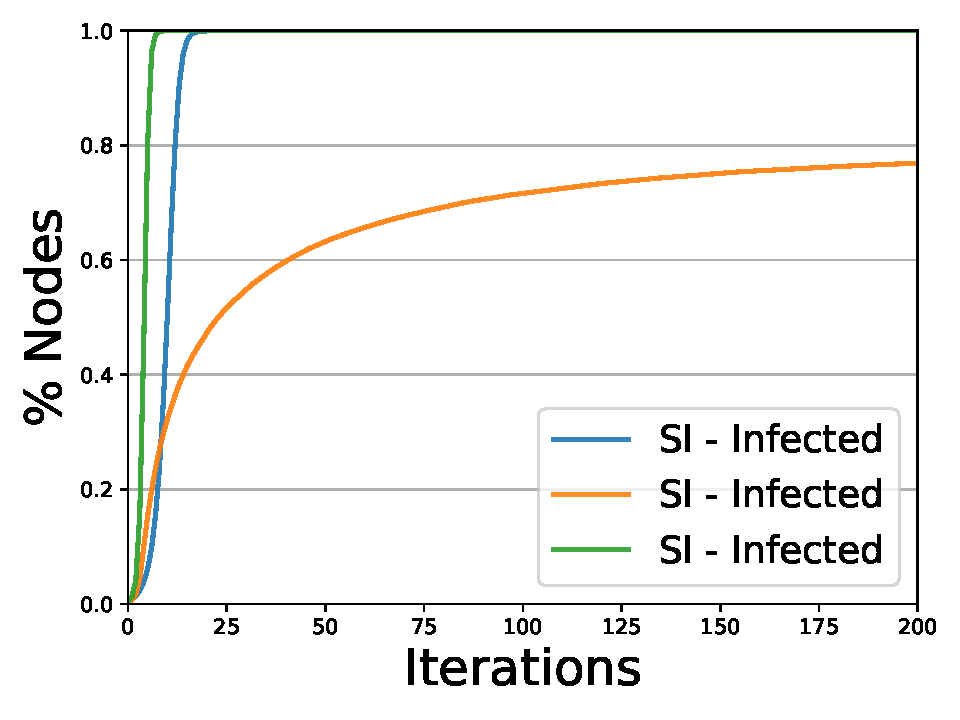
\includegraphics{images/spreading/si/trend_comparison.pdf}
            }
            \caption{}
            \label{diff_si_comparison}
        \end{subfigure}
        \caption{In Figure \ref{diff_si} we can see the diffusion graph for the original network, while in Figure
        \ref{diff_si_er} and in Figure \ref{diff_si_ba} we can see the diffusion graph for the Erdős–Rényi and
        Barabási–Albert networks, respectively. In Figure \ref{diff_si_comparison} we can see a comparison between
        the infection rate of the three networks.}
        \label{diff_si_total}
    \end{figure}
    For the \textbf{Susceptible-Infected} model we've started with a $0.005\%$ of the total population ($3$ nodes)
    of each network being infected, and we've choosed a value of $0.01$ for the infection rate $\beta$. As you can
    see from Figure \ref{diff_si_total}, the original network is the only one that doesn't reach the saturation
    regime, while the other networks reach it within the first $25$ iterations of the model. This is due to the fact
    that both the Erdős–Rényi and the Barabási–Albert network are extremely connected, hence it is more easy for the
    infection to spread among the nodes. For this model we obtain that the \textbf{fraction of infected individuals}
    increases in time as
    \begin{equation*}
        i = \frac{i_0 e^{\beta<k>t}}{1 - i_0 + i_0 e^{\beta<k>t}} = \frac{3 e^{0.38t}}{65726 + 3 e^{0.38t}},
    \end{equation*}
    and the \textbf{characteristic time} required to reach $\frac{1}{e}$ fraction of all susceptible individuals is
    \begin{equation*}
        \tau = \frac{1}{\beta<k>} = \frac{1}{0.38} = 2.63.
    \end{equation*}

% section si_model (end)

\section{SIS model} % (fold)
\label{sec:sis_model}
    \begin{figure}[H]
        \centering
        \begin{subfigure}{0.45\textwidth}
            \resizebox{\textwidth}{!}{
                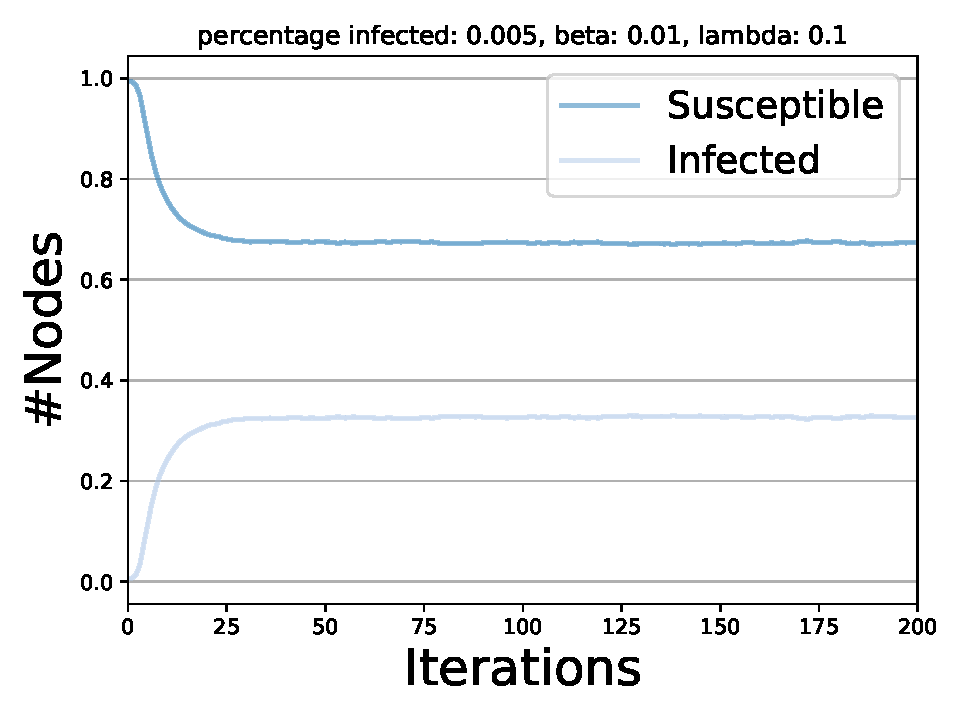
\includegraphics{images/spreading/sis/diffusion.pdf}
            }
            \caption{}
            \label{diff_sis}
        \end{subfigure}
        \begin{subfigure}{0.45\textwidth}
            \resizebox{\textwidth}{!}{
                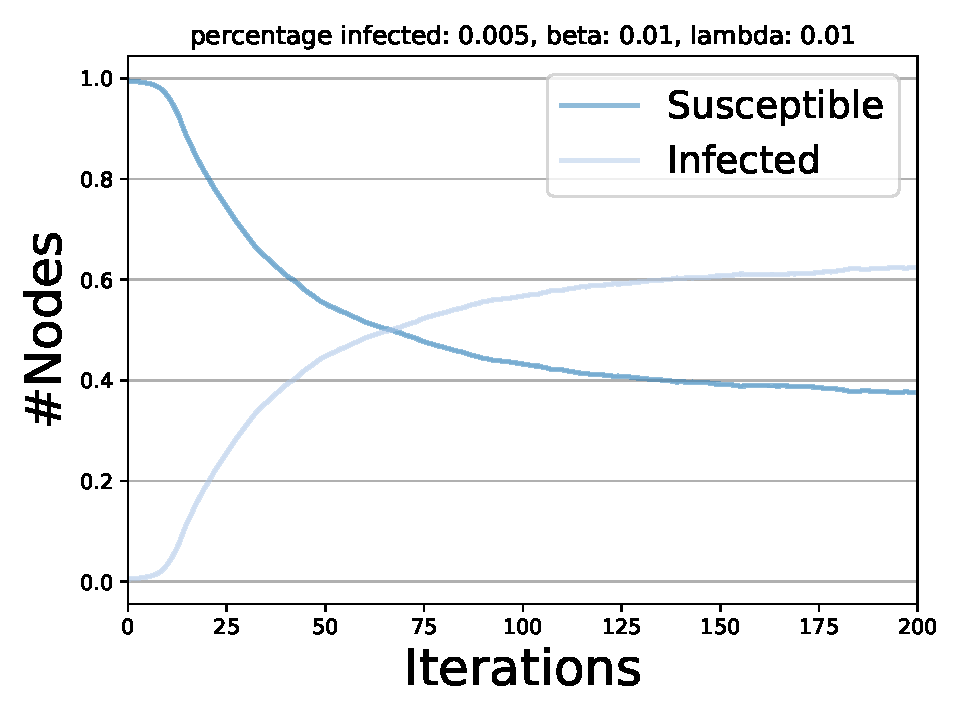
\includegraphics{images/spreading/sis/diffusion_er.pdf}
            }
            \caption{}
            \label{diff_sis_er}
        \end{subfigure}
        \begin{subfigure}{0.45\textwidth}
            \resizebox{\textwidth}{!}{
                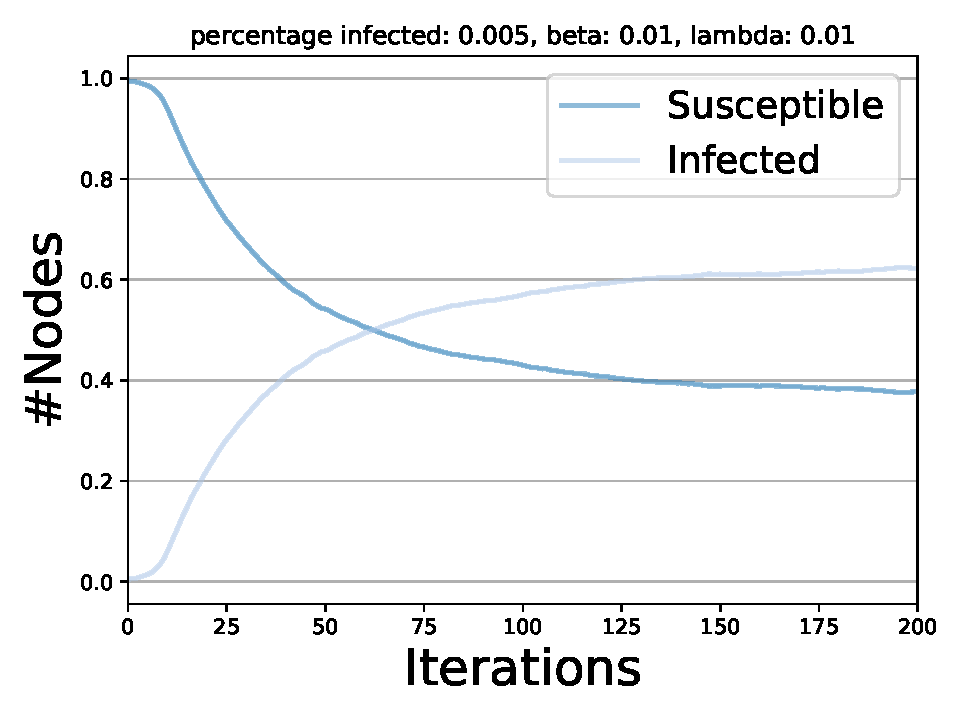
\includegraphics{images/spreading/sis/diffusion_ba.pdf}
            }
            \caption{}
            \label{diff_sis_ba}
        \end{subfigure}
        \begin{subfigure}{0.45\textwidth}
            \resizebox{\textwidth}{!}{
                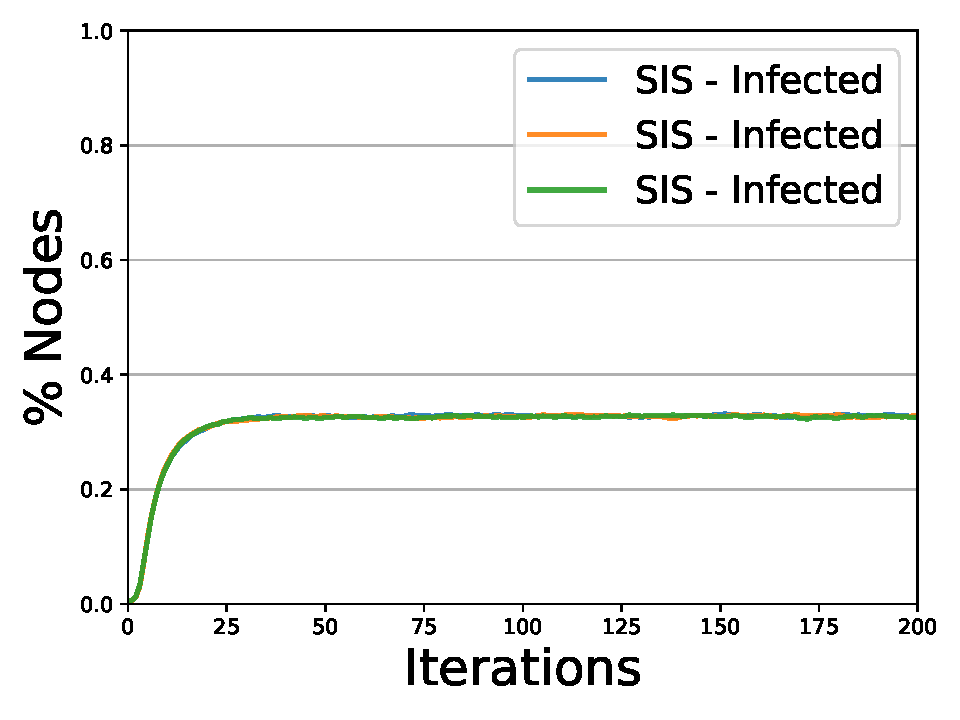
\includegraphics{images/spreading/sis/trend_comparison.pdf}
            }
            \caption{}
            \label{diff_sis_comparison}
        \end{subfigure}
    \end{figure}
% section sis_model (end)

\section{SIR model} % (fold)
\label{sec:sir_model}

% section sir_model (end)

\section{Threshold model} % (fold)
\label{sec:threshold_model}

% section threshold_model (end)
